% Drawing 142/06-17 -- folder 142, batch 06, archive page 116 (PDF page 117).
% Transcription: En bas à gauche, un morceau de carte : le triangle $r$ entre les sommets $0$, $1$, $\infty$ (deux exemplaires de $0$, deux de $1$, deux de $\infty$ sur les bords) ; sommets proches $R^{0,1}_r$, $R^{1,\infty}_r$, $R^{\infty,0}_r$, $R^{0}_{\tau_1 r}$, $R^{1\infty}_{\tau_0 r}$, $R^{\infty,0}_{\tau_0 r}$ ; arcs $\lambda^0_r$, $\lambda^1_r$, $\lambda^\infty_r$, $\lambda^0_{\tau_1 r}$, $\lambda^1_{\tau_0 r}$, $\lambda^\infty_{\tau_0 r}$ ; et les doubles crans $\Lambda^0_r$, $\Lambda^1_r$, $\Lambda^\infty_r$ en arcs courbes autour des sommets.
% Kind: piece of a map with barycentric subdivision (triangle r and neighbours). Method 2 (schematic redraw from the facsimile). Status: partial.
% Notes: The triangle r between the vertices 0, 1, infinity of a piece of map (pencil); the nearby points R^{0,1}_r, R^{1,infty}_r, R^{infty,0}_r, R^0_{tau_1 r}, R^{1 infty}_{tau_0 r}, R^{infty,0}_{tau_0 r}; the arcs lambda and the double notches Lambda as curved arrows round the vertices. Inked arrows drawn schematically; several small labels near infinity are overinked and are placed as the transcription reads them. Only one vertex 0, two 1 and one infinity are clearly visible on the crop (the transcription has two copies of each).
% Coordinates: 1 unit = 1 mm = 1/100 of the crop width (bbox in page fractions: [0.092, 0.646, 0.444, 0.816]).
% Redrawn by Claude (claude-opus-5-5), issue #73, 2026-11-07; not checked by a human; not compiled (no TeX in the session).
% Rights: reproduces part of the work -- behind RENDER_TRANSCRIPTS, never published by itself.
\documentclass[tikz,border=3pt]{standalone}
\usepackage{amsmath,amssymb}
\usetikzlibrary{patterns,arrows.meta}
\tikzset{pencil/.style={black!45}, struck/.style={black!35}, mark/.style={circle,draw,inner sep=1.3pt}, pt/.style={circle,fill,inner sep=0.9pt}, opt/.style={circle,draw,fill=white,inner sep=1.1pt}}
\begin{document}
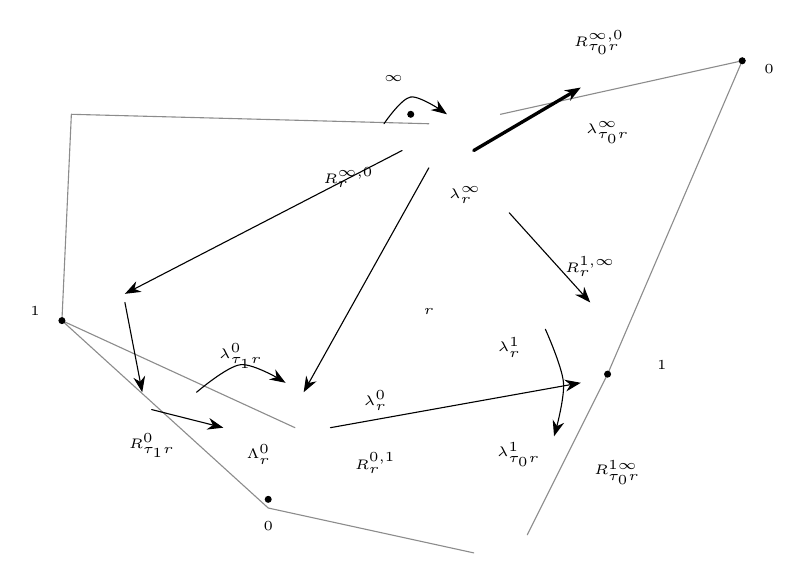
\begin{tikzpicture}[x=1mm,y=1mm,line cap=round,line join=round,font=\scriptsize]
\draw[pencil] (8,-13.6) -- (53.4,-14.8);
\draw[pencil] (8,-13.6) -- (6.8,-39.8);
\draw[pencil] (6.8,-39.8) -- (33,-63.6);
\draw[pencil] (62.5,-13.6) -- (93.2,-6.8);
\draw[pencil] (93.2,-6.8) -- (76.1,-46.6);
\draw[pencil] (76.1,-46.6) -- (65.9,-67);
\draw[pencil] (33,-63.6) -- (59.1,-69.3);
\draw[pencil] (6.8,-39.8) -- (36.4,-53.4);
\node[pt] at (51.1,-13.6) {};
\node[pt] at (93.2,-6.8) {};
\node[pt] at (6.8,-39.8) {};
\node[pt] at (76.1,-46.6) {};
\node[pt] at (33,-62.5) {};
\draw[-{Stealth[length=2mm]}] (53.4,-20.4) -- (37.5,-48.9);
\draw[-{Stealth[length=2mm]}] (40.9,-53.4) -- (72.7,-47.7);
\draw[-{Stealth[length=2mm]}] (63.6,-26.1) -- (73.9,-37.5);
\draw[-{Stealth[length=2mm]}] (50,-18.2) -- (14.8,-36.4);
\draw[-{Stealth[length=2mm]}] (14.8,-37.5) -- (17,-48.9);
\draw[-{Stealth[length=2mm]}] (18.2,-51.1) -- (27.3,-53.4);
\draw[-{Stealth[length=2mm]}] plot[smooth, tension=0.55] coordinates {(23.9,-48.9) (29.5,-45.4) (35.2,-47.7)};
\draw[-{Stealth[length=2mm]}] plot[smooth, tension=0.55] coordinates {(68.2,-40.9) (70.5,-47.7) (69.3,-54.5)};
\draw[very thick,-{Stealth[length=2mm]}] (59.1,-18.2) -- (72.7,-10.2);
\draw[-{Stealth[length=2mm]}] plot[smooth, tension=0.55] coordinates {(47.7,-14.8) (51.1,-11.4) (55.7,-13.6)};
\node[inner sep=1pt] at (48.9,-9.1) {\tiny $\infty$};
\node[inner sep=1pt] at (96.6,-7.9) {\tiny $0$};
\node[inner sep=1pt] at (3.4,-38.6) {\tiny $1$};
\node[inner sep=1pt] at (83,-45.4) {\tiny $1$};
\node[inner sep=1pt] at (33,-65.9) {\tiny $0$};
\node[inner sep=1pt] at (53.4,-38.6) {\tiny $r$};
\node[inner sep=1pt] at (75,-4.5) {\tiny $R^{\infty,0}_{\tau_0 r}$};
\node[inner sep=1pt] at (76.1,-15.9) {\tiny $\lambda^\infty_{\tau_0 r}$};
\node[inner sep=1pt] at (43.2,-21.6) {\tiny $R^{\infty,0}_r$};
\node[inner sep=1pt] at (58,-23.9) {\tiny $\lambda^\infty_r$};
\node[inner sep=1pt] at (73.9,-32.9) {\tiny $R^{1,\infty}_r$};
\node[inner sep=1pt] at (63.6,-43.2) {\tiny $\lambda^1_r$};
\node[inner sep=1pt] at (64.8,-56.8) {\tiny $\lambda^1_{\tau_0 r}$};
\node[inner sep=1pt] at (77.3,-59.1) {\tiny $R^{1\infty}_{\tau_0 r}$};
\node[inner sep=1pt] at (29.5,-44.3) {\tiny $\lambda^0_{\tau_1 r}$};
\node[inner sep=1pt] at (18.2,-55.7) {\tiny $R^0_{\tau_1 r}$};
\node[inner sep=1pt] at (31.8,-56.8) {\tiny $\Lambda^0_r$};
\node[inner sep=1pt] at (46.6,-57.9) {\tiny $R^{0,1}_r$};
\node[inner sep=1pt] at (46.6,-50) {\tiny $\lambda^0_r$};
\end{tikzpicture}
\end{document}
